\section{Resultat}
\label{sec:Lieth_Wahid-results}
I detta avsnitt presentars resultaten som har fåtts från datainsamlingen \ref{ds}.
\subsection{Scrum-utvärdering under sprintuvärdering}
Frågor som ställdes i utvärdering av Scrum \ref{Lieth:scrumU} lade stor fokus på de två viktiga aspekter av Scrum som nämndes tidigar under \ref{two} vilka är transparens och granskning.
Transparens är mycket viktig del av Scrum och därför det togs hänsyn till. Alla medlemmar i teamet var överens om att Scrumbräda som kom i form av ett Trello-Board gjorde det lättare att veta vilka 
utvecklingsuppgifter tilldelades till vilka. Vidare teamet kände sig nöjd med resultaten av stort sett varje sprint. Svaren på \ref{f3} varierade från sprint till annan. Till exempel i början av sprint 2 var väldigt få av teamet  
vana vid JavaScrip, React och all andra essentiella utvecklingsverktyg som behövdes för utföring av projektet. Detta ledde till att tidsuppskattning var dels överskattade och dels underskattad. Teamet bestämde sig redan från
början att hålla öppenhet och transparens d.v.s. om någon i teamet känner sig osäker på att han kan klara en uppgift så kommer teamet hjälpa honom. All kodning som skrevs skickades till Github och där granskades av den automatiserad testnings verktygen \textit{Travis} men också av en av teamets medlemmar.

\subsection{Frågeformulär}
Målet med frågeformuläret var att få en klar bild på vad teamet har fått för erfarenheter från att jobba agilt med Scrum, och vilka delar som är essentiella som behöver vara med för ett framgångsrikt studentprojekt. Först och främst behöver man veta om teamet har kunskap inom Scrum teori därför ställdes frågan \textit{Hade du erfarenheter inom Scrum sedan tidigare? }Resultat av svaren på denne fråga visade att mer hälften av teamet inte hade några erfarenheter av att använda Scrum \ref{q1-4} medan resten inte kände sig bekväma med att använda ramverket. Detta innebär kunskapen inom Scrum utvecklades under projektets gång. Men givet att teamet hade en tidsbudget på 400 timmar per person samt antal uppgifter som behövde utföras därför lades mindre fokus på Scrum och mer på själva utvecklingen.  

Utöver det tyckte 71\% av teamet att Scrum har bidragit att hjälpa oss att jobba effektivare. Detta visar att teammedlemmarna är nöjda med valet av utvecklingsmetodiken vilket visar att Scrum bemötte vår behoven. Å andra sidan varierade svaren när det kom till att beskriva sina upplevelser av jobba Agilt med Scrum. Mer än hälften av teamet beskrev det som positivt trots svårigheter som teamet har haft för att anpassa sig till Scrum vid början av projektet. Resten av svaren var en blandning av att sprinten var allt för korta eller att Scrum inte har hjälpt speciellt mycket. Anledning till detta blir klarare när man kollar på nästa frågan som handlar om vilka delar av Scrum saknades. De flesta tyckte att delar som \textit{stå-upp möten} hade  hjälpt teamet att jobba eff. Vidare tyckte teamet inte att Scrum var nödvändig för projektets framgång dels för att den inte följdes bra av teamet och dels på grund av vi använde väldigt små delar av Scrum till exempel Scrum-bräde.

\begin{figure*}[h]
	\centering
	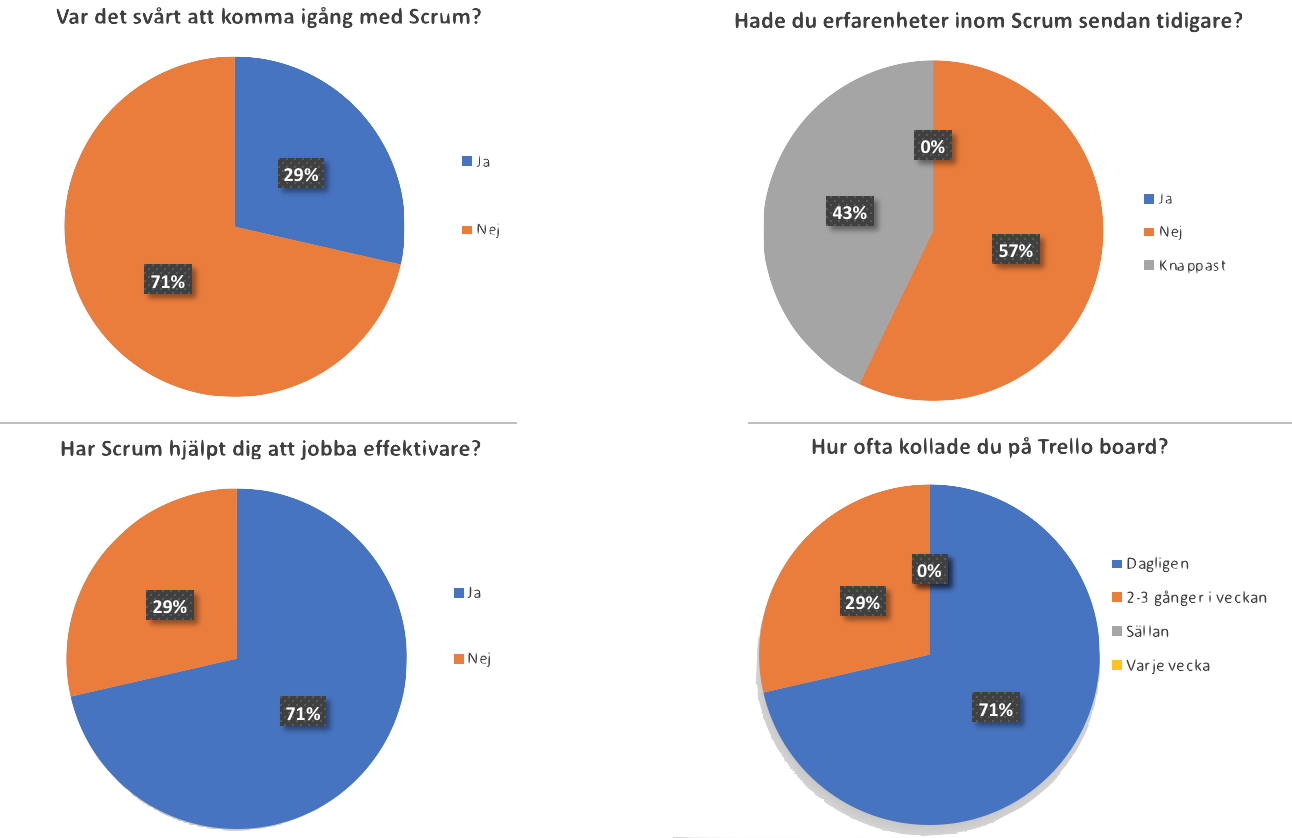
\includegraphics[scale=0.5]{q1-4}
	\caption{Resultat från frågeformuläret}
	\label{q1}
\end{figure*}